
\documentclass[12pt]{book}
\usepackage{listings}
\usepackage{xcolor}

\usepackage{amsmath}
\usepackage{svg}
%New colors defined below
\definecolor{codegreen}{rgb}{0,0.6,0}
\definecolor{codegray}{rgb}{0.5,0.5,0.5}
\definecolor{codepurple}{rgb}{0.58,0,0.82}
\definecolor{backcolour}{rgb}{0.95,0.95,0.95}

%Code listing style named "mystyle"
\lstdefinestyle{mystyle}{
  backgroundcolor=\color{backcolour},   commentstyle=\color{codegreen},
  keywordstyle=\color{blue},
  numberstyle=\tiny\color{codegray},
  stringstyle=\color{codepurple},
  basicstyle=\ttfamily\footnotesize,
  breakatwhitespace=false,         
  breaklines=true,                 
  captionpos=b,                    
  keepspaces=true,                 
  numbers=left,                    
  numbersep=5pt,                  
  showspaces=false,                
  showstringspaces=false,
  showtabs=false,                  
  tabsize=2
}

% %"mystyle" code listing set
\lstset{style=mystyle}
\usepackage[margin=1in]{geometry} 
\usepackage{amsmath,amsthm,amssymb}
\usepackage{graphicx}
\usepackage{float}
\usepackage{blindtext}
\usepackage{pst-node}
\usepackage{pdfpages}

\usepackage{pst-plot}
\usepackage{svg}
\usepackage{amsmath}
\newcommand{\N}{\mathbb{N}}
\newcommand{\Z}{\mathbb{Z}}

\newenvironment{theorem}[2][Theorem]{\begin{trivlist}
\item[\hskip \labelsep {\bfseries #1}\hskip \labelsep {\bfseries #2.}]}{\end{trivlist}}
\newenvironment{lemma}[2][Lemma]{\begin{trivlist}
\item[\hskip \labelsep {\bfseries #1}\hskip \labelsep {\bfseries #2.}]}{\end{trivlist}}
\newenvironment{exercise}[2][Exercise]{\begin{trivlist}
\item[\hskip \labelsep {\bfseries #1}\hskip \labelsep {\bfseries #2.}]}{\end{trivlist}}
\newenvironment{problem}[2][Problem]{\begin{trivlist}
\item[\hskip \labelsep {\bfseries #1}\hskip \labelsep {\bfseries #2.}]}{\end{trivlist}}
\newenvironment{question}[2][Question]{\begin{trivlist}
\item[\hskip \labelsep {\bfseries #1}\hskip \labelsep {\bfseries #2.}]}{\end{trivlist}}
\newenvironment{corollary}[2][Corollary]{\begin{trivlist}
\item[\hskip \labelsep {\bfseries #1}\hskip \labelsep {\bfseries #2.}]}{\end{trivlist}}

\newenvironment{solution}{\begin{proof}[Solution]}{\end{proof}}

\begin{document}
 
% --------------------------------------------------------------
%                         Start here
% --------------------------------------------------------------
 
\title{Pricing Modeling Notes}
\author{\\ %replace with your name
} %if necessary, replace with your course title
 
\maketitle
 
% \begin{theorem}{x.yz} %You can use theorem, exercise, problem, or question here.  Modify x.yz to be whatever number you are proving
% Delete this text and write theorem statement here.
% \end{theorem}
 
% \begin{proof} %You can also use solution in place of proof.
% Blah, blah, blah.  Here is an example of the \texttt{align} environment:
%Note 1: The * tells LaTeX not to number the lines.  If you remove the *, be sure to remove it below, too.
%Note 2: Inside the align environment, you do not want to use $-signs.  The reason for this is that this is already a math environment. This is why we have to include \text{} around any text inside the align environment.


\chapter{Risk Based Pricing}
\section{ Preliminary definitions} 
We will start by characterizing the payouts for a constant installment loan under the assumption that there is no risk. In this world, there is only the contractual cash-flow and no risk of any kind (e.g. prepayment risk, default risk,etc). In section (1.3) we will introduce those risk factors from first principles.
\footnote{The reader familiarized with modern mathematical asset pricing will recognize the similarity of this approach with the typical Q and P measure approach, - i.e. studying first the asset price under a risk neutral world (measure Q) and then connecting with the real world which is non-risk-neutral (P measure) }
\\
\\
The connection between the risk free world and the real world will be established through the theorem of telescopic amortizations in section (1.3). To the best of my knowledge, this theorem has not been established anywhere else but it turns out to be extremely useful for two reasons: First, using this theorem we can easily establish a closed form mathematical representation of the Economic Profit of a loan from first principles even allowing for different modeling choices for the sequence of computations. 
\\ 
\\
Second, the use of the theorem allow for such a simple representation that its programmatic implementation does not need any for-loops of any kind, freeing the space for using the vectorization approach that is widely used in data intensive applications in statistics and deep learning.

\begin{figure}[H]
  \centering
      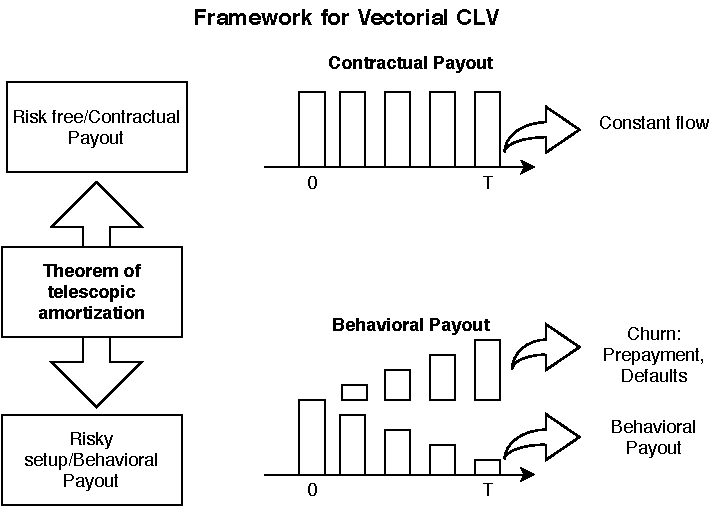
\includegraphics[width=1\textwidth]{ProofDiagram.pdf} 
 \caption{Vectorial setup}
 \label{fig:Test2}
\end{figure}
Finally lets state some basic notation for rates, discount factors and maturity.

\renewcommand{\arraystretch}{1.5} % <-- optional a
\begin{center} % <-- optional b
\begin{math} % <-- step a
\begin{array}{|l|c|l|} \hline % <-- steps b, c; optional c, d
\mbox{Element} & \mbox{Notation}\\ \hline
\mbox{Client Interest Rate}  & r \\
\mbox{Cost of Funds Rate,Fund Transfer Pricing FTP, TT   }  & r_c \\
\mbox{Discount Rate }  & r_d\\
\mbox{Contractual Maturity }  & T \\
\hline
\end{array} % <-- step e
\end{math}% <-- step e
\end{center}



%Page on setup equations
\section{Payment schedule in a risk free world}
\subsection{The Constant Installment Function}
We can define a $c_f(.)$ function to compute constant installments by defining the following equality involving $c$ (the constant installments), $\bar{B}(1)$ (the lended principal), $r$ (the loan interest rate) and $T$ the contractual maturity.
\begin{align}
    \bar{B}(1) &= \frac{c}{(1+r)}+\frac{c}{(1+r)^2}+\frac{c}{(1+r)^3}+...+\frac{c}{(1+r)^T}
\end{align}
Setting $\delta=\frac{1}{1+r}$
\begin{align}
    \bar{B}(1) &=c\delta[1+\delta+\delta^2+\delta^3+\delta^4+...+\delta^{T-1}] \nonumber \\
    &=c\delta\left[\frac{1}{1-\delta}-\delta^T\frac{1}{1-\delta}\right] =c\delta\left(\frac{1-\delta^T}{1-\delta}\right)
\end{align}
Solving for $c$ we establish the definition for $c_f(r,T)$
\begin{align}
    c=\bar{B}(1)\left(\frac{1-\delta}{\delta}\right)\frac{1}{1-\delta^T}=B(1)\left[r\frac{(1+r)^T}{(1+r)^T-1}\right]
\end{align}

\begin{align}
    \boxed{c_f(r,T):=\frac{r(1+r)^T}{(1+r)^T-1}} \implies c=\bar{B}(1)c_f(r,T) \label{eq:c}
\end{align}
\subsection{The Balance Function: }
The Current Balance function $\bar{B}(t)$ is the remaining balance left at time $t-1$ for a loan with principal $B=\bar{B}(1)$ and in absence of any prepayment or default risk \footnote{The acute reader will notice that the definition of $\bar{B}(t)$, in terms of the remaining balance left at time $t-1$ , was given so that we can state such a simple equation for the earned contractual interest $\bar{I}(t)=r\bar{B}(t)$ and eliminate dependence on past indexes $t$.}. For a constant installments loan, the remaining balance at time $t$ for a loan with principal (Balance at t=0) B is given by 
\begin{align}
\bar{B}(t)&=B\frac{(1+r)^T-(1+r)^{t-1}}{(1+r)^T-1} \label{eq:bbar0}
\end{align}

To establish equation (\ref{eq:bbar0}) we start from first principles noticing that 
the remaining balance is the capitalized previous balance minus the installment 

\begin{align}
\bar{B}(t)=\bar{B}(t-1)(1+r)-c \label{eq:bbar2}
\end{align}
Equation (\ref{eq:bbar2}) is a difference equation of first order that can be solved recursively with initial value given by the principal $B$ as follows:
% \begin{align}
% \bar{ I}(t)&=r\times \bar{ B}(t)
% \end{align}
% \paragraph{Constant amortization: } The remaining balance at time $t$ for a loan with principal (Balance at t=0) B is given by:

% \begin{align}
% \bar{B}(t)&=B \times (1-\frac{t-1}{T})
% \end{align}
\begin{align}
    \bar{B}(1)&=B \nonumber \\
    \bar{B}(2)&=\bar{B}(1)(1+r)-c = \bar{B}(1+r)-c \nonumber \\
    \bar{B}(3)&=\bar{B}(2)(1+r)-c = \bar{B}(1+r)^2-c(1+r)-c \nonumber \\
    \bar{B}(4)&=\bar{B}(3)(1+r)-c = \bar{B}(1+r)^3-c(1+r)^2-c(1+r)-c \nonumber \\
    \bar{B}(5)&=\bar{B}(4)(1+r)-c = \bar{B}(1+r)^4-c(1+r)^3-c(1+r)^2-c(1+r)-c \nonumber 
\end{align}  
\begin{align}
    \bar{B}(t)&= \bar{B}(1+r)^{t-1}-c \sum_{s=0}^{t-2} (1+r)^s 
\end{align}
Using the fact that: If $S_n = 1+x+x^2+x^3+...+x^n \implies  S_n=\frac{1-x^{n+1}}{1-x}$
\begin{align}
    \bar{B}(t)&= \bar{B}(1+r)^{t-1}-c \left[ \frac{(1+r)^{t-1}-1}{r} \right]  \label{eq:bprev}
\end{align}
Replacing (\ref{eq:c}) in (\ref{eq:bprev})

\begin{align}
    \bar{B}(t)=\bar{B}(1)\left[ \frac{(1+r)^T-(1+r)^{t-1}}{(1+r)^T-1} \right]
\end{align}
\begin{align}
    \boxed{B_f(t,r,T)=\left[ \frac{(1+r)^T-(1+r)^{t-1}}{(1+r)^T-1} \right]} \implies \bar{B}(t)=\bar{B}(1)B_f(t,r,T)
\end{align}
% \begin{align}
%     \bar{I}(t) = r\bar{B}(1)B_f(t,r,T)
% \end{align}
\subsection{Amortization factor:}
Finally, we define the amortization factor noticing the constant installment should be equal to the interest payment plus the amortization.

\begin{equation}
    A_f(t,r,T) = c_f(r,T)-rB_f(t,r,T) \label{eq:af1}
\end{equation}
\begin{align}
    \boxed{A_f(t,r,T)=\frac{r(1+r)^{t-1}}{(1+r)^T-1}} \label{eq:afactor}
\end{align}
\begin{corollary}{1}
Using (\ref{eq:bbar2}) and (\ref{eq:af1}) we can state that:
\[
1-\sum_{s=1}^{t-1} A_f(s,r,T)=B_f(t)
\]
\end{corollary} 

\section{Introducing Risk Events in Payment schedule}
Last section we defined financial math operators to define a loan payment schedule in absence of any risk events. In this section we introduce risk events including defaults and prepayments. Lets start with the Theorem of Telescopic Amortizations which will be key to connect the risk free schedule with the risky schedule.
\begin{theorem}{1.1 (Telescopic Amortizations)}{} \label{teo:1}
If A is the function defined in (\ref{eq:afactor}) then:
\[
\prod^{t-1}_{s=1}(1-A_f(1,r,T-s+1))=1-\sum^{t-1}_{s=1}A_f(s,r,T) =B_f(t,r,T)
\]
\end{theorem}

\begin{proof}{}{} Lets define
\[
E_1=\prod^{t-1}_{s=1}(1-A_f(1,r,T-s+1)), \\
E_2 =1-\sum^{t-1}_{s=1}A_f(s,r,T)
\]
and
\[
\delta =1/(1+r)
\]
Working on $E_1$ and setting $\xi=1+r$:
\begin{align}
1-A_f(1,r,T-s+1) = \frac{(1+r)^{T-s+1}-1-r}{(1+r)^{T-s+1}-1}=\frac{\xi^{T-s+1}-\xi}{\xi^{T-s+1}-1} \nonumber
\end{align}

\begin{align}
\implies E_1 =& \frac{(\xi^T-\xi)}{(\xi^T-1)}\times \frac{(\xi^{T-1}-\xi)}{(\xi^{T-1}-1)} \times \frac{(\xi^{T-2}-\xi)}{(\xi^{T-2}-1)} \times ... \times \frac{(\xi^{T-t+1}-\xi)}{(\xi^{T-t+1}-1)} \nonumber\\
=&\xi^t \frac{(\xi^{T-1}-1)}{(\xi^T-1)}\times \frac{(\xi^{T-2}-1)}{(\xi^{T-1}-1)} \times \frac{(\xi^{T-3}-1)}{(\xi^{T-2}-1)} \times ... \times \frac{(\xi^{T-t}-1)}{(\xi^{T-t+1}-1)} \nonumber\\
=&\frac{\xi^T-\xi^t}{\xi^T-1} \label{eq:e1}
\end{align}

Working on $E_2$:
\begin{align}
A_f(s,r,T) = \frac{r(1+r)^{s-1}}{(1+r)^{T}-1}=(\xi-1)\frac{\xi^{s-1}}{\xi^{T}-1} \nonumber
\end{align}

\begin{align}
\implies E_2 =& 1-\frac{(\xi-1)(1+\xi+\xi^2+\xi^3+...+\xi^{t-1})}{\xi^T-1}\nonumber\\
=&\frac{\xi^T-\xi^t}{\xi^T-1} 
\end{align}
$\therefore E1=E2$\\
Finally, the second equality follows directly from Corollary 1.
\end{proof}

\subsection{Default and Prepayment probabilities and the survival function:}
We define de conditional probabilities $p_p(t)$ and $p_d(t)$ $\forall t \in \{1,2,...T\}$ as follows:
\begin{align}
   p_p(t)  :&  \mbox{
   Probability that the loan will prepay at time t given that it has survived to that point } \nonumber \\
   p_d(t)  : &  \mbox{
   Probability that the loan will default at time t given that it has survived to that point 
   } \nonumber
\end{align} \noindent
 Given these definitions we can establish $S(t)$, the probability that a loan survives until period $t$ using the pigeon hole principle. 
\begin{align}
S(t) & = (1-p_d(1) - p_p(1))\times(1-p_d(2) - p_p(2))\times...\times(1-p_d(t) - p_p(t)) \nonumber\\ 
 & =  \Pi_{s=1}^t (1-p_d(s) - p_p(s))  
\end{align}



%  Page on setup examples
\section{Alternative setups for Incremental Profit computation}



\subsection{Standard model \label{can}} 
In this model prepayments/full prepayment, default probability are expressed as conditional probabilities. This probabilities are conditioned on the running active balance i.e. the balance that has not been prepaid or defaulted upon.
\begin{figure}[H]
  \centering
      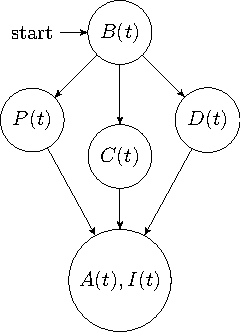
\includegraphics[width=.3\textwidth]{Graph2.pdf} 
 \caption{Computation Graph}
 \label{fig:graph2}
\end{figure}

\begin{center} % <-- optional b
%\[ % <-- step a
\begin{math}
\begin{array}{|l|c|l|} \hline % <-- steps b, c; optional c, d
\mbox{Variable} &\mbox{Notation} & \mbox{Calculation}\\ \hline
\mbox{Balance in presence of risk }  & B(t)  & B(t)\\
\mbox{Default  }  & D(t) & p_d(t) B(t)\\
\mbox{Full Prepayment}  & C(t) & p_c(t) B(t)\\
\mbox{Prepayment  }  & P(t) & p_p(t)B(t)\\
\mbox{Amortization}  & A(t) &(B(t)-D(t)-C(t)-P(t)) A_f(1,r,T-t+1)\\
\mbox{Interest }  & I(t) & (B(t)-D(t)-C(t)-P(t))r\\
\mbox{Principal   }  &  B(1) & B\\
\mbox{Risky balance next period   }  &  B(t+1) & B(t)-D(t)-C(t)-P(t)-A(t)\\
\hline
\end{array} % <-- step e
%\] % <-- step e
\end{math}
\captionof{table}{Computation for Model 1: Standard Model} \label{table:1}
\end{center}

Notice that we defined $B(t)$ as the Loan Balance subject to risk (Behavior affected Loan Balance), as opposed to $\bar{B}(t)$, which is the Risk Free Loan Balance (Contractual Balance).  Given this definitions we can compute the recursive form for the balance function $B(t)$
\begin{align}
B(t+1) =& B(t)[1-p_d(t)-p_c(t)-p_p(t)-(1-p_d(t)-p_c(t)-p_p(t))A_f(1,r,T-t+1) ] \nonumber\\
     =&
    B(t)(1-p_d(t)-p_c(t)-p_p(t))(1-A_f(1,r,T-t+1)) \label{eq:bbar1}\
\end{align}


Notice that (\ref{eq:bbar1}) is a first order equation in difference which can be easily solved as.
\begin{align}
    B(t) =\prod^{t-1}_{s=1} (1-A_f(1,r,T-s+1))(1-p_d(s)-p_c(s)-p_p(s))B
\end{align}
Using theorem (\ref{teo:1}) we can state the behavioral balance $B(t)$ as a function of the contractual balance.
\begin{align}
    B(t) &=\prod^{t-1}_{s=1} (1-p_d(s)-p_c(s)-p_p(s))\bar{B}(t) \nonumber\\
    &=S(t-1)\bar{B}(t) \nonumber
\end{align}
\begin{align}
    \boxed{B(t)=S(t-1)\bar{B}(t) } \label{eq:model1}
\end{align}
Equation \ref{eq:model1} states a very simple relation between the theoretical/contractual balance $\bar{B}(t)$ and the behavioral balance $B(t)$. We have derived this equation from a first principles approach through the Theorem of Telescopic Amortization (\ref{teo:1}). This equation represent a very powerful shortcut not only for using intuition, since the behavioral balance can be thought of as the contractual balance adjusted by the survival probability, but also for implementing the model programatically using vectorization instead of recursive loops over the different points in the payment schedule, the last alternative can be very hard to maintain and compute, not to mention its proneness to error.
\begin{corollary}{: Interest in model 1}
Given the interest rate definition in Table (\ref{table:1}) and equation (\ref{eq:model1}) we can state that:
\begin{align}
    \boxed{I(t)=S(t)\bar{B}(t)r}
\end{align}


\end{corollary}

\subsection{Prepayment dependent on initial balance}
This model is a variation of the previous one in which the prepayment probability is a proportion of the initial balance/principal $B(1)$. In this setup, the prepayment amount will be define in function of the marginal probability of default $p^m_p(t)$ and not the conditional probability $p_p(t)$ 
\begin{figure}[H]
  \centering
      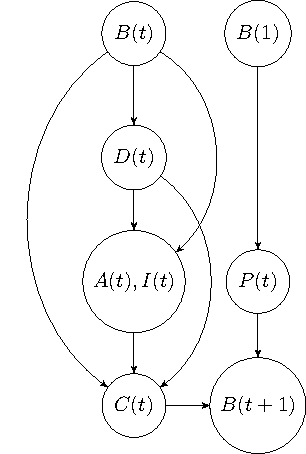
\includegraphics[width=.3\textwidth]{Graph1.pdf} 
 \caption{Computation Graphs: Model 2}
 \label{fig:Test}
\end{figure}

\begin{center} % <-- optional b
% \[ % <-- step a
\begin{math}
\begin{array}{|l|c|l|} \hline % <-- steps b, c; optional c, d
\mbox{Variable} &\mbox{Notation} & \mbox{Calculation}\\ \hline
\mbox{Balance in presence of risk }  & B(t)  & B(t)\\
\mbox{Default  }  & D(t) & p_d(t) B(t)\\
\mbox{Amortization}  & A(t) &(B(t)-D(t)) A_f(1,r,T-t+1)\\
\mbox{Interest }  &  I(t) & (B(t)-D(t))r\\
\mbox{Full Prepayment}  & C(t) & p_c(t) [B(t)-D(t)-A(t)]\\
\mbox{Principal   }  &  B(1) & B\\
\mbox{Prepayment  }  & P(t) & p_p^m(t)B\\
\mbox{Risky balance next period  }  & B(t+1) & B(t)-D(t)-C(t)-P(t)-A(t)\\
\hline
\end{array} % <-- step e
\end{math}
% \] % <-- step e
\captionof{table}{Computation for Model 2: Prepayment Dependent on Initial Balance} 
\end{center}

  Given this definitions we can compute the recursive form for the balance function $B(t)$
\begin{align}
\scriptstyle
     B(t+1) =&\scriptstyle B(t)[1-p_d(t)-p_c(t)(1-p_d(t)-(1-p_d(t))A_f(1,r,T-t+1))-(1-p_d(t))A_f(1,r,T-t+1) ]-p_p^m(t) B(1) \nonumber\\
    =&\scriptstyle B(t)[1-p_d(t)-p_c(t)+p_d(t)p_c(t)+p_c(t)(1-p_d(t)A_f(1,r,T-t+1)-(1-p_d(t))A_f(1,r,T-t+1)]
    -p_p^m(t) B(1) \nonumber\\
    =&\scriptstyle
    B(t)[ (1-p_d(t))(1-p_c(t))-(1-p_d(t))(1-p_c(t))A_f(1,r,T-t+1)]
    -p_p^m(t) B(1) \nonumber\\
     =&\scriptstyle
    B(t)(1-p_d(t))(1-p_c(t))(1-A_f(1,r,T-t+1))
    -p_p^m(t) B(1) \label{eq:bbar}\
\end{align}
Notice that (\ref{eq:bbar}) is a first order equation in difference of type $x(t+1) = \alpha(t)x(t) + \beta(t)$  where $\alpha(t):=(1-p_d(t))(1-p_c(t))(1-A_f(1,r,T-t+1))$  , $\beta(t):= -p_p^m(t) \bar{B}(1)$, $x(t):= \bar{B}(t)$ and the initial condition given by the lended principal $x(1) = \bar{B}(1) = B$. This equation can be easily solved as: 
\begin{align}
    x(t) = x_1 \prod_{s=1}^{t-1} \alpha(s) + \sum_{k=1}^{t-2} \left[\beta(k) \prod_{s=k+1}^{t-1}\alpha(s)\right]+\beta(t-1)
\end{align}
Plugging back the definitions of $\alpha(t)$, $\beta(t)$ and ,$x(t)$ we get:
\begin{align}
    B(t) =&\prod^{t-1}_{s=1} (1-p_d(s))(1-p_p(s))(1-A_f(1,r,T-s+1))B \nonumber\\
            &-\sum_{k=1}^{t-2}\left[p_p^m(k) B \prod_{s=k+1}^{t-1}(1-p_d(s))(1-p_c(s))(1-A_f(1,r,T-s+1))\right]-p_p^m(t-1) B
\end{align}
Using the theorem of Telescopic Amortizations (\ref{teo:1}) and defining $\Tilde{S}(t):=\Pi_{s=0}^t(1-p_d(s))(1-p_c(s))$ we can state the behavioral balance $B(t)$ as a function of the contractual balance $\bar{B}(t)$.
\begin{align}
    B(t) &=\Tilde{S}(t-1)\bar{B}(t)-\sum_{k=1}^{t-2} \left[ p_p^m(k)B \frac{\Tilde{S}(t-2) }{\Tilde{S}(k) }  \frac{ \bar{B}(t-1)}{ \bar{B}(k+1)}\right] -p_p^m(t-1) B\nonumber\\
    &=\Tilde{S}(t-1)\bar{B}(t)-\sum_{k=1}^{t-1} \left[ p_p^m(k)B \frac{\Tilde{S}(t-1) }{\Tilde{S}(k) }  \frac{ \bar{B}(t)}{ \bar{B}(k+1)}\right] \nonumber  \\
    &=\Tilde{S}(t-1)\left(1-\sum_{k=1}^{t-1}   \frac{p_p^m(k)B }{\Tilde{S}(k) \bar{B}(k+1)} \right)\bar{B}(t) \nonumber 
\end{align}
We define conveniently $S(t)$ as:
\begin{align}
S(t-1):=\Tilde{S}(t-1)\left(1-\sum_{k=1}^{t-1}   \frac{p_p^m(k)B }{\Tilde{S}(k) \bar{B}(k+1)} \right)^{+}  \label{eq:model3}
\end{align}
So that we can state that:
\begin{align}
    \boxed{B(t)=S(t-1)\bar{B}(t)  } \label{eq:model2}
\end{align}
Equation (\ref{eq:model3}) is analogous to equation (\ref{eq:model1}) with an additional term that represents a weighted sum of the last prepayment amounts where the last prepayment has a weight of one. 
\section{ Terms included in the incremental profit (CLV)}
\subsection{ Interest on loans: }
Independently of the model, we saw that $B(t) = S(t-1)\bar{B}(t)$ so given any of the computations graphs we can state.
\begin{align}
LI(t) = S(t)\bar{ B}(t)r \label{eq:li}
\end{align}


\subsection{  Cost of Funds: }
This term represents the amount of balance the lender has to finance through the cost of funds $r_c$. We follow the setup suggested by Phillips (2018):
\begin{align}
COF(t) = S_c(t)\bar{ B}_c(t)r_c
\end{align}
where: 
\begin{align}
S_c(t)= \Pi_{s=0}^t [1- p_p(s)-(1-LGD(s))p_d(s) ]
\end{align}
This setup assumes that, if the client prepays, the bank also prepays the remaining capital that is owed. If the client defaults, the bank uses the recovered capital (i.e.$(1-LGD(t))$) to make a prepayment to the remaining owed capital and still has to keep making interest payments on the amount defaulted. \\

Think about this scenario in the following way: At each time, there are three possible states of nature that will determine the remaining balance next period: 1) The client does not default nor prepays with probability $(1-p_p(t)-p_c(t))$, in this case the remaining balance is still B(t), 2) The client prepays with probability $p_p(t)$, thus the bank prepays an the remaining balance and the banks due balance becomes zero, 3) The client defaults with probability $p_d(t)$, thus the bank pays back only $(1-LGD(t) \times  B(t)$ (which means the bank will not need to make interest payments for that capital anymore) but it will still have to make interest payments for the capital amount equal to $LGD(t) \times B(t)$. It follows that the expected value of the remaining balance will be $(1-p_p(t)-(1-LGD(t))p_d(t))B(t)$.
\footnote{ 
Observe that if we state
\begin{align}
    COF(t) = S(t)\bar{B}_c(t)r_c
\end{align}
the ALM unit will have to fund the behavioral expected balance, i.e the remaining balance after deducting prepayments (either full or partial) and defaults. However in this case we would be missing the interest payments that the ALM has to make for the part that could not be recovered at default (i.e. $LGD(t) \times B(t)$) since it has to payback the borrowed funding  

}
\subsection{ Equity Benefit (Capital Rebate) and Equity Capital Charge: }
Since any loan has to be financed by both debt and capital, let's assume the fraction of capital the lender has to maintain for each lended dollar is $\alpha_t$. To be consistent with the left and right side of the balance sheet, we need to take into account both the additional revenue of investing the amount of required capital (Equity Benefit) and also the equity charge that the shareholder demands.

\begin{align}
EB(t) = \alpha_t S(t)\bar{ B}(t) r_c
\end{align}
\begin{align}
 EC(t) =  \alpha_t S(t)\bar{ B}(t) r_e
\end{align}

\subsection{ Loss from Default: }
So far, we have included the effect of the client's behavior on the interest income and outcome. In this term, we will also incorporate the loss of capital in which the lending entity incur when a client defaults. 
\begin{align}
EL(t) =  p_d(t)LGD(t)S(t)\bar{ B}(t) 
\end{align}

\subsection{ Fees and Servicing Costs: }
The lending entity can get additional source of revenue or incur in costs that do not depend on the lended amount can be written as:
\begin{align}
F(t) = f S(t)
\end{align}
\begin{align}
SC(t) =  \sigma S(t)
\end{align}


\subsection{Recovery costs}
In case of default the bank recovers an amount of capital equal to $(1-LGD(t)) \times B(t)$ which the bank uses to prepay the funding used to back the loan as we saw in section ()
\begin{align}
C(t) = c\times p_d(t) S(t)
\end{align}



\section{ Incremental Profit Definition (CLV): }
Following Phillips 2018 \cite{phillips-2018}. We define the incremental value for a credit as follows:

\renewcommand{\arraystretch}{1.5} % <-- optional a
\begin{center} % <-- optional b
\[ % <-- step a
\begin{array}{|l|c|l|} \hline % <-- steps b, c; optional c, d
\mbox{Element} & \mbox{Notation} & \mbox{Calculation}\\ \hline
\mbox{Lending Interest }  & LI & PV(LI(t),r_d,T)\\
\mbox{Cost of Funds   }  & COF & PV(COF(t),r_d,T)\\
\mbox{Equity benefit }  & EB & PV(EB(t),r_d,T)\\
\mbox{Fees }  & LI & PV(F(t),r_d,T)\\
\mbox{Ancillary profit }  & A & -\\
\mbox{Origination cost}  & OC & -\\
\mbox{Commision  }  & COM & -\\
\mbox{Servicing Costs}  & SC & PV(SC(t),r_d,T)\\
\mbox{Expected Loss }  & EL & PV(EL(t),r_d,T)\\
\mbox{Collection costs }  & C & PV(C(t),r_d,T)\\
\mbox{Equity charge}  & EC & PV(EC(t),r_d,T)\\

\hline
\end{array} % <-- step e
\] % <-- step e
\end{center}

\renewcommand{\arraystretch}{1.5} % <-- optional a
\begin{center} % <-- optional b
\[ % <-- step a
\begin{array}{|l|c|l|} \hline % <-- steps b, c; optional c, d
\mbox{Element} & \mbox{Notation} & \mbox{Calculation}\\ \hline
\mbox{Net Interest Income }  & NII & LI-COF+EB\\
\mbox{Total Income  }  & TI & NII+A+F\\
\mbox{Net Income before tax}  & NIBT & TI-OC-COM-SC-LD-C\\
\mbox{Net Income after tax }  & NIAT&(1-\tau)\times NIBT \\
\mbox{Incremental profit  }  & IP & NIAT-EC\\

\hline
\end{array} % <-- step e
\] % <-- step e
\end{center}
Where 
\begin{align}
PV(x(t),r_d,T)=\sum_{t=1}^T \frac{x(t)}{(1+r_d)^t}
\end{align}

\subsection{ Incremental Profit Function: }
Define the incremental profit function as:
\begin{align}
\pi(p)=IP(p,r_d,B,T,\theta) \label{eq:IP}
\end{align}

Given definition (\ref{eq:IP}) we can perform several types of computations. For example, to compute the IRR of a given rate $p$ we set $IP(p,irr,B,T,\theta)=0$. To compute the minimun rate that covers all costs (and risks) and yields a profitability of $r_d$ we set $IP(r^{min},r_d,B,T,\theta)=0$. Notice that given this setup, charging the minimum rate does not mean the lending entity is not making money, it just means we are charging enough to reach a target profitability rate.


\chapter{Willingness to Pay Modeling (WTP): }
\section{The Price-Response Function}
Each price-response function specifies the demand that the lender would experience at each price, which will depend on:
\begin{enumerate}
    \item Total number of clients interested in the loan
    \item Number of applicant clients
    \item The number of applicant the lender deems creditworthy and quotes a price.
    \item Number of accepted applicants who would achieve a positive surplus from taking the loan from the lender at the offered price.
    \item Number of accepted applicants who \textbf{take-up} the offered loan.
\end{enumerate}
In most lending markets, the final price is not known to the client at the time she applies for the loan so we assume that the number of clients who apply for a loan is not influenced by the price.
\begin{align}
d(p)=D\bar{F}(p) \label{eq:demand}
\end{align}
$d(p)$ is the number of the loans offered by a lender that would be taken up at the price p. $D$ is the number of successful applicants for the loan, and $\overline{F}(p)$ is the take-up rate, which is defined as the fraction of successful applicants who will take up the loan at price $p$

\begin{align}
\bar{F}(p)=\int^\infty_p f(w)dw
\end{align}
\section{Segmented vs Join Estimation \label{sec:takeuprate}}
For $n$ segments, the segmented estimation assumes each segments has its own demand function so we need to estimate $2n$ parameters.
\begin{align}
\bar{F_i}(p_i)=\frac{e^{a_i+b_i p_i}}{1+e^{a_i+b_i p_i}}
\end{align}

For $n$ segments, the join estimation assume we can estimate one single price price response function that includes all explanatory variables within it (including price)
\begin{align}
\bar{F}(p_i,a,b,\theta,x_i)=\frac{e^{a+b p_i+\theta^T x_i}}{1+e^{a+b p_i+\theta^T x_i}}
\end{align}
\chapter{Price optimization (CLV+WTP): }
\section{Price optimization without constraints}
\begin{align}
p^*= \arg \max_p \sum_{i=1}^N D_i\overline{F}_i(p_i)\pi(p)
\end{align}

\section{Price optimization with competing objectives: The efficient Frontier}

\begin{align}
p^*_j= \arg \max_p \sum_{i=1}^N D_i\bar{F}_i(p_i)\pi(p)
\end{align}
\begin{center}
    $s.t.$
\end{center}
\begin{align}
\sum_{i=1}^N D_i\bar{F}_i(p_i) =q_j,& \forall j
\end{align}
\chapter{Survival models}
\subsection{Common survival setup}
Let T be a positive random variable in $1,2,3,...$
\begin{align}
    S(t)=&P(T>t) \\
    F(t)=&1-S(t)=1-P(T>t)=P(T\leq t)
\end{align}
\subsection{Survival setup in presence of competing risks}

We define the cumulative incidence function as:
\begin{align}
    CIF_k(t)=&P(T\leq t,D=k) \\
    &=\sum_k P(T \leq t,D=k) = P(T \leq t)
\end{align}
In order to see what is the relationship between the CIF function and the usual conditional probability of default (death) we state the definition of conditional probability and use the fact that the event $T=t+1 \wedge T>t$ is equal to $T=t+1$ standalone.
\begin{align}
    p_k(t+1)&=p(T=t+1,D=k/T>t)=\frac{P(T=t+1,D=k)}{P(T>t)}\\
    &= \frac{ P(T \leq t+1,D=k)-P(T\leq t,D=k)}{
    1-\sum_k P(T \leq t, D=k)
    }
\end{align}

As an example lets consider that $D=1$ represents default
and $D=2$ represents prepayment then the conditional probabilities of default and prepayment are given by:
\begin{align}
p_d(t+1)&= \frac{CIF_d(t+1)-CIF_d(t)  }{
1- CIF_d(t)-CIF_p(t)}  
\end{align}


% \title{Inkscape package on Overleaf }
\chapter{The PricingPy Python Library}
\section{Implementation in vectorial form}
In the previous chapter we showed the full model and expressed in such a simple final equation that it can be stated directly in vectorial form in Python or any programatic language with support for matrix algebra.\\

For ilustration purposes, consider the computation given in equation (\ref{eq:bbar1}). To implemet that we will define the following vectors:
\begin{align}
T = \begin{bmatrix} 
    T_{1} & \dots &  T_{m} \\
    \end{bmatrix}    
\end{align}
\begin{align}
r = \begin{bmatrix} 
    r_{1} & \dots &  r_{m} \\
    \end{bmatrix}    
\end{align}
\begin{align}
disb = \begin{bmatrix} 
    d_{1} & \dots &  d_{m} \\
    \end{bmatrix}    
\end{align}
\begin{align}
T^{mat} = \begin{bmatrix} 
     1  \\
     2  \\
    \vdots  \\
    T^{max} 
    \end{bmatrix}       
\end{align}
With the definitions above, $\bar{B}$ can be diretly computed using equation (\ref{eq:bbar1}) and array broadcasting operators in numpy:

\begin{align}
    \bar{B} = disb*\frac{(1+r)^{T^{max}}-(1+r)^{T^{mat}-1}}{(1+r)^{T^{max}}-1}
\end{align}
With this approach $\bar{B}$ results of order $T^{max}\times m$ as expected.
\begin{align}
\bar{B} = \begin{bmatrix} 
    b_{1,1} & \dots &  b_{1,m} \\
    \vdots & \ddots & \\
    b_{T^{max},1} &        & b_{T^{max},m} 
    \end{bmatrix}    
\end{align}
\section{Class Diagram}
\begin{figure}[H]
  \centering
      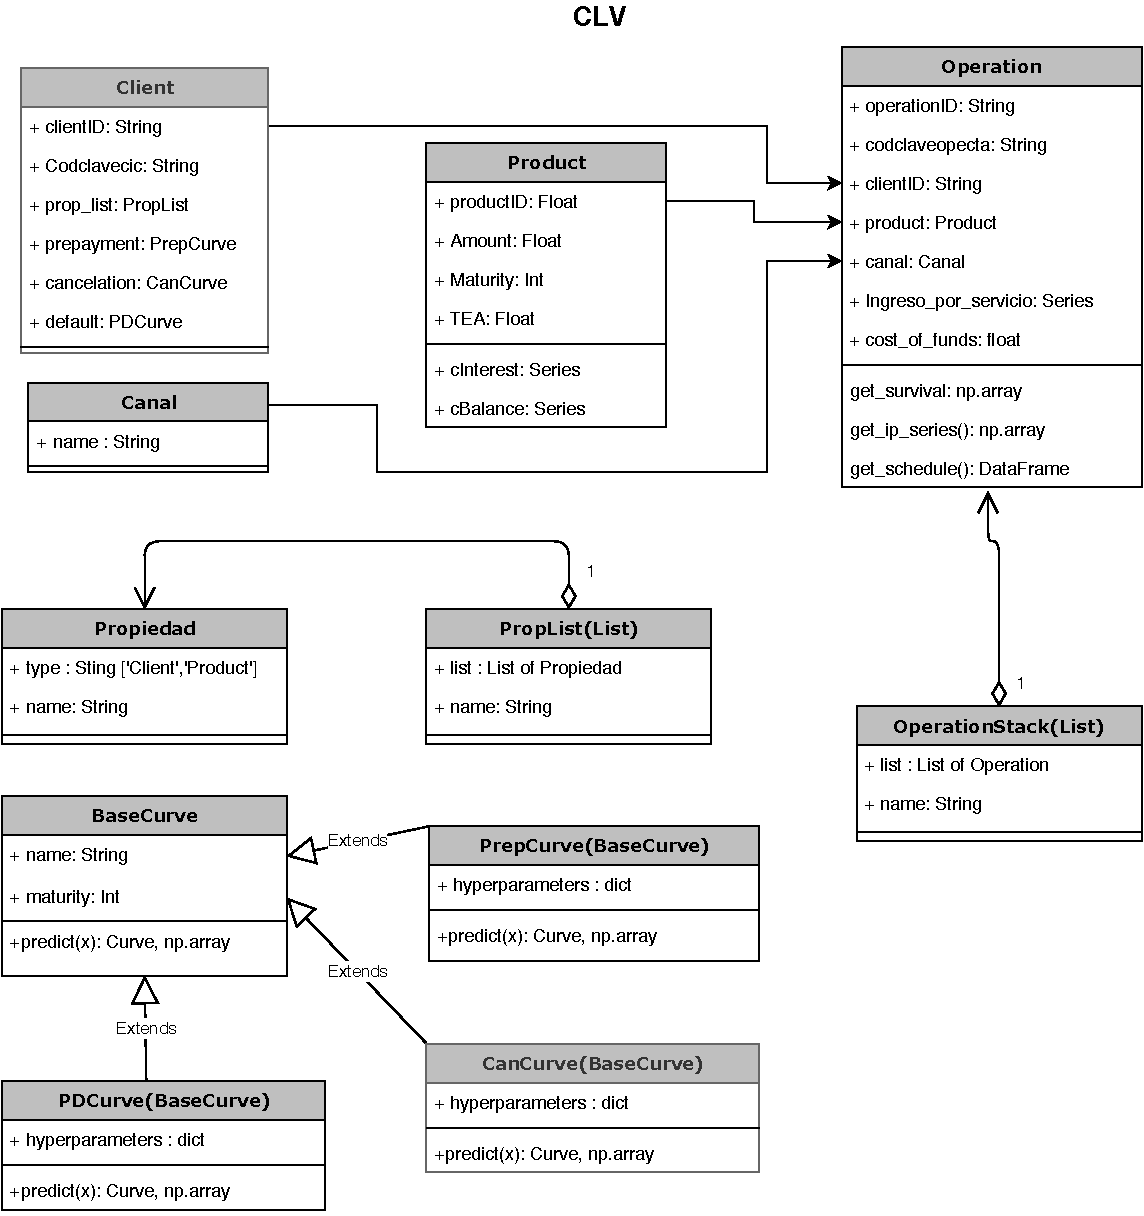
\includegraphics[width=1\textwidth]{diagrCLV.pdf} 
 \caption{CLV Class Diagram}
 \label{fig:Test}
\end{figure}

\begin{figure}[H]
  \centering
      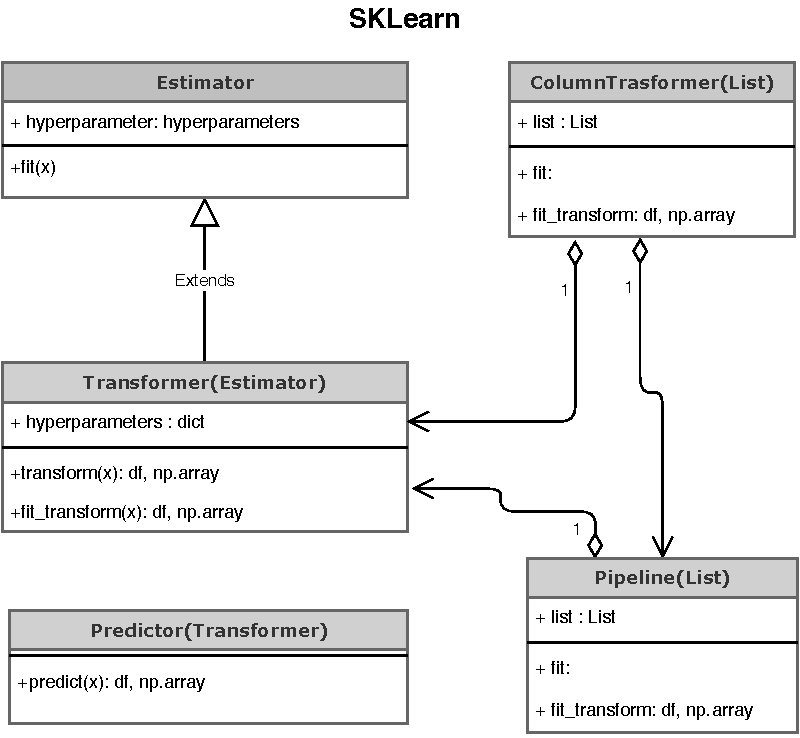
\includegraphics[width=.6\textwidth]{diagrSklearn.pdf} 
 \caption{SKLearn Class Diagram}
 \label{fig:Test}
\end{figure}



%Python code highlighting
\begin{lstlisting}[language=Python, caption=Python example]
import pandas as pd
import numpy as np
import PyPricing as ppr

# Loading Data
filename = 'inputs.xlsx'
full_filename = Path('.').resolve() / 'data'/ filename
X = pd.read_excel(full_filename, sheet_name = 'inputs')

# Creating CLV engine to compute CLV   
eng = ppr.CLVEngine()
Xtr = eng.transform(X) 
eng = eng.predict(Xtr) # computes behavioral curves and update all behavioral curves

# Computations
PV = eng.get_pv()
RMIN = eng.get_rmin()
IRR = eng.get_irr()
SCHED = eng.get_schedule()

\end{lstlisting}

% --------------------------------------------------------------
%     You don't have to mess with anything below this line.
% --------------------------------------------------------------

 
\end{document}